\documentclass{article}
\usepackage{graphicx}
\usepackage{amsmath}
\usepackage[sorting=none]{biblatex}
\addbibresource{manual.bib}

\title{LIFTLINE Manual}
\author{Christopher C. Chinske}

\begin{document}
\maketitle
\newpage
\tableofcontents
\newpage
\section{Introduction}
\paragraph{}
LIFTLINE is a collection of MATLAB scripts and functions that
implement lifting-line theory.  It solves the monoplane equation to
estimate aerodynamic characteristics of a finite wing.  It also
provides capabilities to analyze shear force and bending moment along
the wing spar.
\subsection{Theory}
\paragraph{}
LIFTLINE implements lifting-line theory as described in \cite{bertin}
and \cite{anderson}.  The program estimates the spanwise circulation
of a finite wing.  Following from this result, the program can compute
the lift and vortex-induced drag coefficients.  The program can also
estimate structural characteristics, such as shear and bending moment
along the wing.
\paragraph{}
Classical lifting-line theory assumes incompressible flow, no wing
sweep, and linear airfoil section lift-curve slopes.  Currently,
LIFTLINE assumes:
\begin{enumerate}
\item Incompressible flow
\item No wing sweep (input required to properly draw planform)
\item Linear airfoil section lift-curve slopes
\item Symmetrical loading.
\end{enumerate}
Future versions of LIFTLINE will implement a modified lifting-line
theory and relax these assumptions.
\subsection{Program Organization}
\paragraph{}
The directory scripts\_aircraft contains input scripts that define
wing geometry and structural loads (e.g., fuel or stores).  The
directory scripts\_cases contains input scripts that define case
parameters.  These parameters may be overridden for certain analyses.
\subsection{Concept of Operations}
\paragraph{}
When analyzing a wing of finite span, the primary goals are to
determine: spanwise circulation, spanwise lift distribution, lift
coefficient, and vortex-induced drag coefficient.  Other goals might
include finding shear and bending moment for a cantilever wing,
determining rolling and yawing moments (for asymmetric loading), or
determining the stalling angle of attack.  The general procedure for
carrying out this analysis using LIFTLINE is outlined below.
\begin{enumerate}
\item Build an input script (aircraft) that defines the wing geometry.
\item Plot and verify the planform geometry.
\item Build an input script (case) that defines case parameters.
\item Run a grid convergence analysis, and update the case script.
\item For level flight, find the angle of attack for L = W, and update
  the case script.
\item Run case for a particular angle of attack to get spanwise
  circulation, spanwise lift distribution, lift coefficient, and
  vortex-induced drag coefficient.
\end{enumerate}
If desired, the lift and vortex-induced drag coefficients can be
computed across a range of angles of attack.  The spar shear and
bending moment can also be computed.
\paragraph{}
The function LIFTLINEUI provides an interactive user interface, which
aids the user in executing many of these tasks.
\paragraph{}
Advanced users can also call any of the program's library functions
directly.  In this way, users can build custom analysis routines.  The
figure below graphically depicts a typical workflow.
\newline
\newline
\fbox{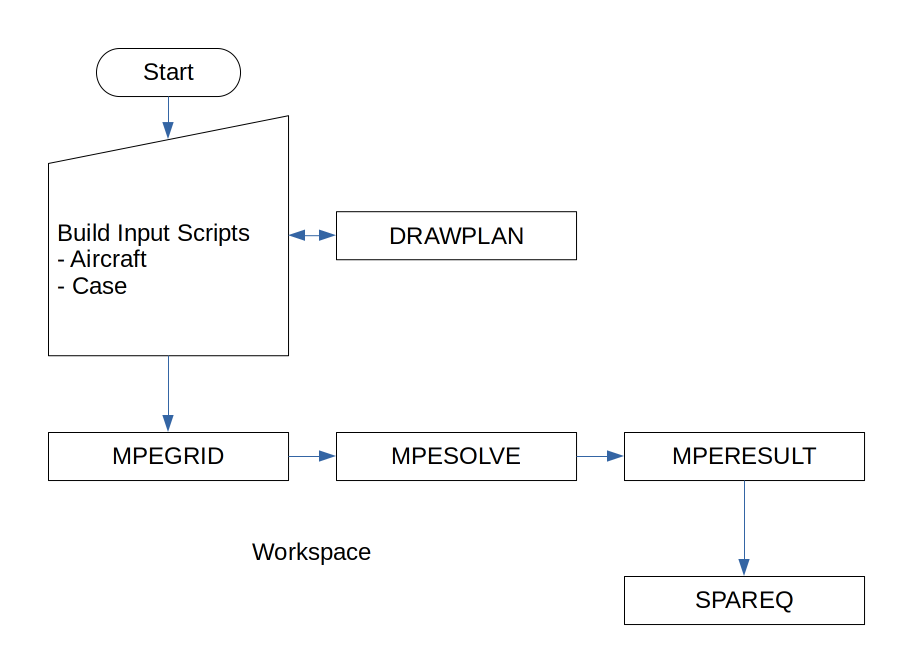
\includegraphics[width=\textwidth]{images/flowchart.png}}
\newline
\newline
\newpage
\printbibliography
\end{document}
